\documentclass[final,3p,times]{elsarticle}

\usepackage{lipsum}
 \usepackage{graphics}
\usepackage[]{algorithm2e}
 \usepackage{setspace}
%% or use the graphicx package for more complicated commands
 \usepackage{graphicx}
%% or use the epsfig package if you prefer to use the old commands
 \usepackage{epsfig}
 \usepackage{subfigure}

%% The amssymb package provides various useful mathematical symbols
\usepackage{amssymb}
%% The amsthm package provides extended theorem environments
 \usepackage{amsthm,amsmath}
 \usepackage{multirow}
 \usepackage{setspace}
 \usepackage{CJK}
 \usepackage{float}
 \usepackage{pdfpages}
 \restylefloat{table}
 \onehalfspacing



\makeatletter
\def\ps@pprintTitle{%
	\let\@oddhead\@empty
	\let\@evenhead\@empty
	\def\@oddfoot{}%
	\let\@evenfoot\@oddfoot}
\makeatother


\begin{document}

\begin{frontmatter}

\title{MATH 6740: Financial Mathematics and Simulation\\
	Homework 1 solutions/presentation}

\author[rvt]{Jubiao ``Jack'' Yang}

\address[rvt]{Rensselaer Polytechnic Institute, Troy, NY 12180}


\end{frontmatter}

\section{Q1}
	The single-period market can be expressed by a $2\times2$ matrix $\mathbf{M}$ and an initial price vector $\mathbf{s}$:
	\begin{subequations}
		\label{EqnDefinitionMs0}
		\begin{equation}
			\mathbf{M}=
				\begin{bmatrix}
					s^u & 1+r \\
					s^d & 1+r
				\end{bmatrix}
			,
		\end{equation}
		\begin{equation}
			\mathbf{s}_0=
				\begin{bmatrix}
					s_0 & 1
				\end{bmatrix}^T
			.
		\end{equation}
	\end{subequations}
	To find an arbitrage for this market, we can attempt to construct a portfolio $\mathbf{x}=\begin{bmatrix} x_1 & x_2 \end{bmatrix}^T$ that costs zero to set up:
	\begin{equation}
		\label{EqnCostZero2x2}
		c=\mathbf{s}_0^T \mathbf{x}= s_0 x_1 + x_2 = 0
		,
	\end{equation}
	while making sure the future value of this portfolio $\mathbf{v}=\mathbf{Mx}$ is nonnegative at either market state and is not zero at both market states:
	\begin{equation}
		\label{EqnPositivePortfolioValue2x2}
		\mathbf{v}=
			\begin{bmatrix}
				v^u & v^d
			\end{bmatrix}^T,\text{ where }
			\begin{cases}
				v^u \geq 0,~v^d \geq 0 \\
				v^u+v^d>0
			\end{cases}
		.
	\end{equation}
	
	According to the information given:
	\begin{equation}
		\label{EqnConditionQ1}
		s^d = s^u < s_0 \left(1+r\right)
		,
	\end{equation}
	the future value of a portfolio $\mathbf{x}$ would be:
	\begin{equation}
		\mathbf{v}=\mathbf{Mx}=
			\begin{bmatrix} s^u & 1+r \\ s^u & 1+r \end{bmatrix}
			\begin{bmatrix} x_1 \\ x_2 \end{bmatrix}
			=
			\begin{bmatrix} s^u x_1 + \left(1+r\right) x_2 \\ s^u x_1 + \left(1+r\right) x_2 \end{bmatrix}
			=
			\left( s^u x_1 + \left(1+r\right) x_2 \right) \begin{bmatrix} 1 \\ 1 \end{bmatrix}
			.
	\end{equation}
	Therefore, to satisfy the conditions set in Equations (\ref{EqnCostZero2x2}) and (\ref{EqnPositivePortfolioValue2x2}), we have:
	\begin{equation}
		\begin{cases}
			s_0 x_1 + x_2 = 0 \\
			s^u x_1 + \left(1+r\right) x_2 > 0
		\end{cases}
		\quad \Rightarrow \quad
		s^u x_1 - \left(1+r\right) s_0 x_1 > 0
		\quad \Rightarrow \quad
		x_1 \left[ s^u - \left(1+r\right) s_0 \right] > 0
		.
	\end{equation}
	Combined with the condition $s^u < s_0 \left(1+r\right)$ given in Equation (\ref{EqnConditionQ1}), an arbitrage for this market is:
	\begin{equation}
		\mathbf{x}=
			\begin{bmatrix} 1 \\ -s_0 \end{bmatrix} x_1, \text{ where } x_1<0
		.
	\end{equation}
	An explicit example is:
	\begin{equation}
		\mathbf{x}=
		\begin{bmatrix} -1 \\ s_0 \end{bmatrix}
		.
	\end{equation}
	
\section{Q2}
	The incomplete market has been described with:
	\begin{equation}
		\begin{aligned}
			\mathbf{M}&=
				\begin{bmatrix}
					1 & 1+r & 1+s \\
					1 & 1+r & 1+s \\
					1 & 1+r & 1+s
				\end{bmatrix},
				\text{ where } 0<r<s<1
				,\\
			\mathbf{s}_0&= \begin{bmatrix} 1 & 1 & 1 \end{bmatrix}^T.
		\end{aligned}
	\end{equation}
	To construct an arbitrage, we build a portfolio $\mathbf{x}=\begin{bmatrix} x_1 & x_2 & x_3 \end{bmatrix}^T$ with
	\begin{equation}
		\mathbf{x}^T \mathbf{s}_0 = x_1+x_2+x_3 = 0
		,
	\end{equation}
	while making sure that the claim vector
	\begin{equation}
		\mathbf{v}=\mathbf{M} \mathbf{x}
		=
		\begin{bmatrix} 1 & 1+r & 1+s \\ 1 & 1+r & 1+s \\ 1 & 1+r & 1+s \end{bmatrix}
		\begin{bmatrix} x_1 \\ x_2 \\ x_3 \end{bmatrix}
		=
		\left[x_1+\left(1+r\right)x_2+\left(1+s\right)x_3\right]
		\begin{bmatrix} 1 \\ 1 \\ 1 \end{bmatrix}
	\end{equation}
	is in the positive octant including its boundaries but excluding the origin. Combining the above 2 equations we have:
	\begin{equation}
		\mathbf{v}=
		\left(r x_2+s x_3\right)
		\begin{bmatrix} 1 \\ 1 \\ 1 \end{bmatrix}
		,
	\end{equation}
	therefore as long as $x_2\geq0, ~x_3\geq0, ~x_2+x_3>0$, we have a portfolio that takes advantage of the arbitrage. An explicit example would be:
	\begin{equation}
		\begin{bmatrix} x_1 \\ x_2 \\ x_3 \end{bmatrix}=
		\begin{bmatrix} -2 \\ 1 \\ 1 \end{bmatrix}
	\end{equation}
	
\section{Q3}
	To ``design'' a $2\times2$ market with uniform risk-neutral probability, we assign value of $1/2$ to both $q_1$ and $q_2$. With $\mathbf{M}$ and $\mathbf{s}_0$ defined by Equation (\ref{EqnDefinitionMs0}), we have:
	\begin{gather}
		\begin{bmatrix} 1/2 & 1/2 \end{bmatrix}
		\begin{bmatrix} s^u & 1+r \\ s^d & 1+r \end{bmatrix}
		=
		\left( 1+r \right)\begin{bmatrix} s_0 & 1 \end{bmatrix},\\
		\Downarrow\nonumber\\
		\label{EqnQ3nn1}
		\begin{cases}
			s^u + s^d = 2\left(1+r\right) s_0 \\
			1+r = 1+r
		\end{cases}.
	\end{gather}
	According to Equation (\ref{EqnQ3nn1}), we can set up such a market $\left(\mathbf{M},\mathbf{s}_0\right)$ with uniform risk-neutral probability with $r=.05$, $s_0=2$, $s^d=1.5$, and $s^u=2.7$:
	\begin{subequations}
		\label{EqnQ3soln}
		\begin{equation}
		\mathbf{M}=
		\begin{bmatrix}
		2.7 & 1.05 \\
		1.5 & 1.05
		\end{bmatrix}
		,
		\end{equation}
		\begin{equation}
		\mathbf{s}_0=
		\begin{bmatrix}
		2 & 1
		\end{bmatrix}^T
		.
		\end{equation}
	\end{subequations}
	
\section{Q4}
	To find in this market a risk-neutral probability vector $\mathbf{q}=\begin{bmatrix} q_1 & q_2 & q_3\end{bmatrix}^T$, such that:
	\begin{subequations}
		\begin{align}
			\begin{split}
				\label{EqnRiskNeutralProbability}
				&\mathbf{q}^T \mathbf{M} = \left( 1+s \right) \mathbf{s}_0^T
				,
			\end{split}\\
			\begin{split}
				&\mathbf{q}>0 \iff q_j>0~\forall j
				.
			\end{split}
		\end{align}
	\end{subequations}
	Equation (\ref{EqnRiskNeutralProbability}) in this case is therefore:
	\begin{gather}
		\begin{bmatrix} q_1 & q_2 & q_3 \end{bmatrix}
		\begin{bmatrix} 1 & 1+r & 1+s \\ 1 & 1+r & 1+s \\ 1 & 1+r & 1+s \end{bmatrix}
		=
		\left(1+s\right) \begin{bmatrix} 1 & 1 & 1 \end{bmatrix},\nonumber\\
		\Downarrow\nonumber\\
		\label{EqnQ2nn1}
		\left( q_1 + q_2 + q_3 \right) \begin{bmatrix} 1 & 1+r & 1+s \end{bmatrix} = \left(1+s\right) \begin{bmatrix} 1 & 1 & 1 \end{bmatrix},\\
		\Downarrow\nonumber\\
		\label{EqnQ2nn2}
		\begin{bmatrix} 1 & 1+r & 1+s \end{bmatrix} = \left(1+s\right) \begin{bmatrix} 1 & 1 & 1 \end{bmatrix}.
	\end{gather}
	The fact that $\sum_{j} q_j = 1$ is employed in the above derivation. Apparently Equation (\ref{EqnQ2nn1}) is unsolvable as $\begin{bmatrix} 1 & 1+r & 1+s \end{bmatrix}$ and $\begin{bmatrix} 1 & 1 & 1 \end{bmatrix}$ are linearly independent given $0<r<s$; Equation (\ref{EqnQ2nn2}) further confirms this by futilely equating $1$ and $1+r$ with $1+s$. Therefore, this incomplete market has no risk-neutral probability vector.
	
\section{Q5}
	A generic $2\times2$ market $\left(\mathbf{M},\mathbf{s}_0\right)$ is defined in Equation (\ref{EqnDefinitionMs0}); that it is arbitrage-free implies that $s^d<\left(1+r\right)s_0<s^u$, and therefore makes it complete by effecting $\mathbf{M}$ to be full-rank. Thus there exists the inverse of $\mathbf{M}$:
	\begin{equation}
		\mathbf{M}^{-1}=\frac{1}{\left(s^u-s^d\right)\left(1+r\right)}
		\begin{bmatrix} 1+r & -\left(1+r\right) \\ -s^d & s^u \end{bmatrix}
		.
	\end{equation}
	
	To meet the contingency claims $\mathbf{v}^{I}=\begin{bmatrix} 1 & 0\end{bmatrix}^T$, $\mathbf{v}^{II}=\begin{bmatrix} 0 & 1\end{bmatrix}^T$, and $\mathbf{v}^{III}=\begin{bmatrix} a & b \end{bmatrix}^T=a\mathbf{v}^{I}+b\mathbf{v}^{II}$, we need to design corresponding portfolios $\mathbf{x}^{I}$, $\mathbf{x}^{II}$, and $\mathbf{x}^{III}$ to hedge against those.
	
	To hedge against $\mathbf{v}^{I}=\begin{bmatrix} 1 & 0\end{bmatrix}^T$:
	\begin{gather}
		\begin{bmatrix} s^u & 1+r \\ s^d & 1+r \end{bmatrix}
		\begin{bmatrix} x^{I}_1 \\ x^{I}_2 \end{bmatrix}
		=
		\begin{bmatrix} 1 \\ 0 \end{bmatrix},\nonumber\\
		\Downarrow\nonumber\\
		\begin{bmatrix} x^{I}_1 \\ x^{I}_2 \end{bmatrix}
		=
		\frac{1}{\left(s^u-s^d\right)\left(1+r\right)}
		\begin{bmatrix} 1+r & -\left(1+r\right) \\ -s^d & s^u \end{bmatrix}
		\begin{bmatrix} 1 \\ 0 \end{bmatrix}
		=
		\frac{1}{\left(s^u-s^d\right)\left(1+r\right)}
		\begin{bmatrix} 1+r \\ -s^d \end{bmatrix}
		.
	\end{gather}
	The cost of this portfolio $\mathbf{x}^{I}$ is:
	\begin{equation}
		c_0^{I}=\mathbf{s}_0^T\mathbf{x}^{I}=\frac{\left(1+r\right)s_0 - s^d}{\left(s^u-s^d\right)\left(1+r\right)}
		.
	\end{equation}
	
	Similarly, to hedge against $\mathbf{v}^{II}=\begin{bmatrix} 0 & 1\end{bmatrix}^T$:
	\begin{gather}
		\begin{bmatrix} s^u & 1+r \\ s^d & 1+r \end{bmatrix}
		\begin{bmatrix} x^{II}_1 \\ x^{II}_2 \end{bmatrix}
		=
		\begin{bmatrix} 0 \\ 1 \end{bmatrix},\nonumber\\
		\Downarrow\nonumber\\
		\begin{bmatrix} x^{II}_1 \\ x^{II}_2 \end{bmatrix}
		=
		\frac{1}{\left(s^u-s^d\right)\left(1+r\right)}
		\begin{bmatrix} 1+r & -\left(1+r\right) \\ -s^d & s^u \end{bmatrix}
		\begin{bmatrix} 0 \\ 1 \end{bmatrix}
		=
		\frac{1}{\left(s^u-s^d\right)\left(1+r\right)}
		\begin{bmatrix} -\left(1+r\right) \\ s^u \end{bmatrix}
		.
	\end{gather}
	The cost of this portfolio $\mathbf{x}^{II}$ is:
	\begin{equation}
		c_0^{II}=\mathbf{s}_0^T\mathbf{x}^{II}=\frac{-\left(1+r\right)s_0 + s^u}{\left(s^u-s^d\right)\left(1+r\right)}
		.
	\end{equation}
	
	To hedge against $\mathbf{v}^{III}=a\mathbf{v}^{I}+b\mathbf{v}^{II}$:
	\begin{equation}
		\mathbf{x}^{III}
		=\mathbf{M}^{-1}\mathbf{v}^{III}
		=\mathbf{M}^{-1}\left(a\mathbf{v}^{I}+b\mathbf{v}^{II}\right)
		=a\mathbf{x}^{I}+b\mathbf{x}^{II}
		,
	\end{equation}
	and the cost of this portfolio is:
	\begin{equation}
		c_0^{III}
		=\mathbf{s}_0^T\mathbf{x}^{III}
		=\mathbf{s}_0^T\left(a\mathbf{x}^{I}+b\mathbf{x}^{II}\right)
		=ac_0^{I}+bc_0^{II}
		=\frac{\left(a-b\right)\left(1+r\right)s_0 + b s^u - a s^d}{\left(s^u-s^d\right)\left(1+r\right)}
		.
	\end{equation}
	
\section{Q6}
	Thanks to the fact that $\mathbf{M}$ is invertible, $\mathbf{q}^T \mathbf{M}=\left(1+r\right)\mathbf{s}_0^T$ yields $\mathbf{q}^T=\left(1+r\right)\mathbf{s}_0^T \mathbf{M}^{-1}$:
	\begin{equation}
		\begin{bmatrix} q_1 & q_2 \end{bmatrix}
		=
		\frac{1}{s^u-s^d}
		\begin{bmatrix} s_0 & 1 \end{bmatrix}
		\begin{bmatrix} 1+r & -\left(1+r\right) \\ -s^d & s^u \end{bmatrix}
		=
		\frac{1}{s^u-s^d}
		\begin{bmatrix} \left(1+r\right)s_0 - s^d \\ -\left(1+r\right)s_0 + s^u \end{bmatrix}^T
		.
	\end{equation}
	
	Therefore the expected value of $\mathbf{v}^{I}=\begin{bmatrix} 1 & 0\end{bmatrix}^T$ is:
	\begin{equation}
		E_{\mathbf{q}}\left[\mathbf{v}^{I}\right]=\mathbf{q}^T \mathbf{v}^{I}
		=\frac{\left(1+r\right)s_0 - s^d}{s^u-s^d}
		,
	\end{equation}
	and the expected value of $\mathbf{v}^{I}=\begin{bmatrix} 1 & 0\end{bmatrix}^T$ is:
	\begin{equation}
		E_{\mathbf{q}}\left[\mathbf{v}^{II}\right]=\mathbf{q}^T \mathbf{v}^{II}
		=\frac{-\left(1+r\right)s_0 + s^u}{s^u-s^d}
		.
	\end{equation}
	
\appendix

\section{Original Homework Questions (attached)}
	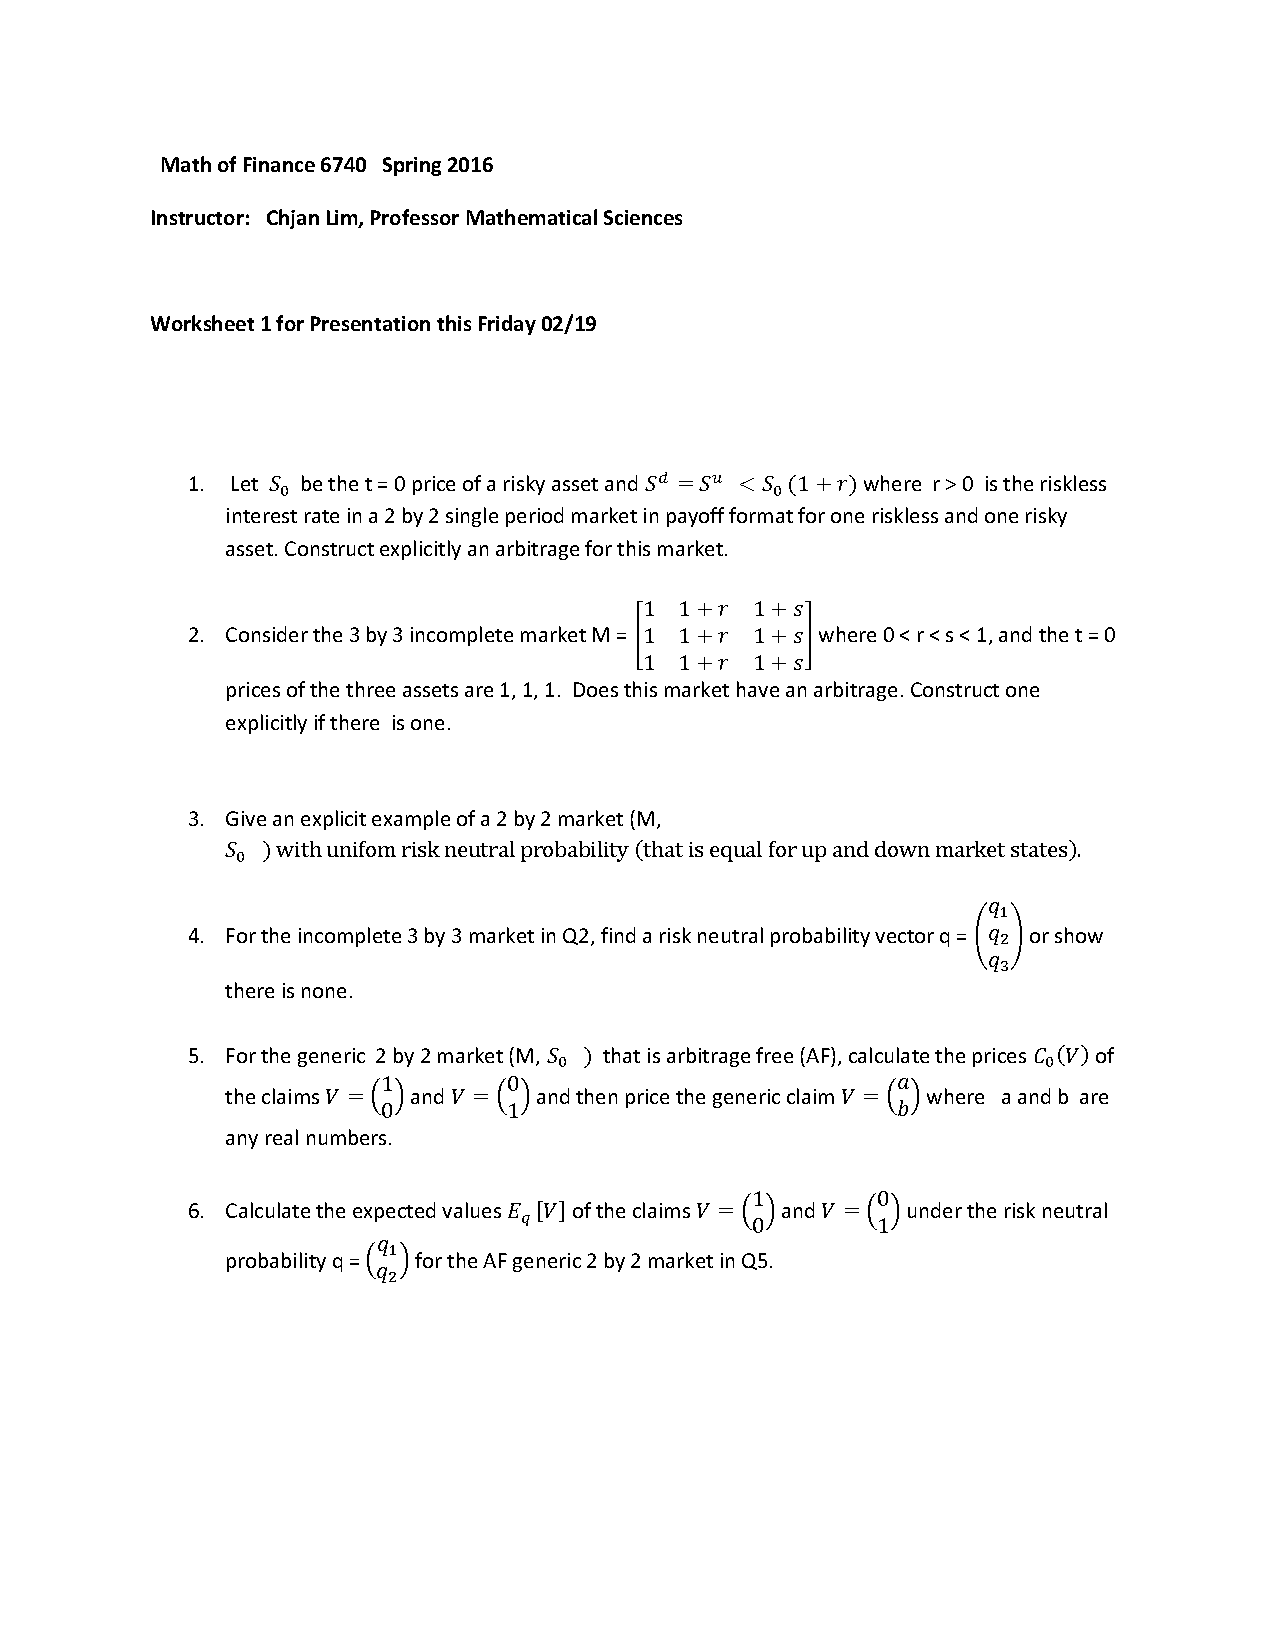
\includepdf[pages={1}]{hwk116a.pdf}


%	\appendix
%%% \section{}
%%% \label{}
%
%%% References
%%%
%%% Following citation commands can be used in the body text:
%%% Usage of \cite is as follows:
%%%   \cite{key}         ==>>  [#]
%%%   \cite[chap. 2]{key} ==>> [#, chap. 2]
%%%
%
%%% References with bibTeX database:
%
%	\section{Reference}
%	\bibliographystyle{elsarticle-num}
%	\bibliography{moptaRefer}
%
%%% Authors are advised to submit their bibtex database files. They are
%%% requested to list a bibtex style file in the manuscript if they do
%%% not want to use elsarticle-num.bst.
%
%%% References without bibTeX database:
%
%% \begin{thebibliography}{00}
%
%%% \bibitem must have the following form:
%%%   \bibitem{key}...
%%%
%
%% \bibitem{}
%
%% \end{thebibliography}

\end{document}



